\setcounter{chapter}{2}
\setchapterabstract{This chapter examines the intersection of antitrust law and economics. Antitrust aims to prevent firms from engaging in practices that harm consumer welfare, primarily by limiting output and increasing prices. While antitrust focuses on firms' conduct, it's important to consider the broader market context, including government regulations and market structures. The chapter discusses the economic concepts of perfect competition, monopoly, and efficiency, and how they inform antitrust analysis. It also highlights the evolving perspectives on antitrust goals and enforcement, with a focus on consumer surplus and long-term effects. The chapter concludes by comparing the European and Chicago School approaches, which differ in their emphasis on consumer welfare versus total surplus.}
\chapter{Goals, Antitrust Provisions, and Economics}
\vspace{-1.5cm}

{\chaptoc\noindent\begin{minipage}[inner sep=0,outer sep=0]{0.9\linewidth}\section{Recap and Agenda}\end{minipage}}

        Antitrust is a set of legal rules (prohibiting arrangements, anticompetitive behaviour and mergers, etc.) aimed at preventing some firms’ practices that may worsen the market well functioning as it result from Consumer Surplus variations.
        
        Three clarifications are needed: (a) Firms’ practices, (b) Market well-functioning, and (c) Market power

    \subsection{Firms' Practices}

        Antitrust rules deal with agreements, monopolistic practices, and mergers, i.e. they address firms’ conduct; not what governments/legislators may decide. Competition law is concerned with restraints of competition started by private parties, not with those restraints compelled by, or effectively controlled by, the government and its branches. Firms are liable as long as they have room to decide their own behaviour; they are not liable for antitrust violations when their practices strictly result from statutes, laws, regulations, or are formally imposed by governments. \\

        A market can be depicted as a circle in which firms are free to play by adopting their business strategies and behavior. The area of the circle can be restricted by the State through laws \& regulations setting the playground, i.e. limiting:
            \begin{itemize}
                \item \textbf{Access conditions} (think at the broadcasting free to air market, train passenger transport)
                \item \textbf{Exit conditions} (think at bank branches, airlines: Alitalia, but also many others etc.), and
                \item \textbf{The rules of the game} (regulation of many aspects: number of flights, spots, air control, safety condition, etc.).
            \end{itemize}
        In other words, firms are not always free to set their strategies, to decide where, how, and how many goods they produce; where, how and at which price they can sell their goods; etc. This may be due to the need to pursue some legitimate goal different from competition (fixing the max. price of protective masks/swabs to avoid speculative behavior by drugstores; limiting sale of alcoholic beverages to minors for health reasons, etc.) However, these restrictive regulations can also be the outcome of lobbies’ pressure or a myopic/interested legislator.

        \subsubsection{Market Structure}

        \Example{
        A very old Italian Law obliged the Italian producers of matches to participate to a Consortium (“Consorzio Italiano Fiammiferi”, C.I.F.), whose goal was inter alia to allocate production/distribution quotas between its members. Furthermore, the law prohibited the distribution in Italy of matches originating from undertakings which did not belong to the Consortium.
        }

        \subsubsection{Thus, hands up?}

            In those markets, the law prevents firms to behave competitively. Undertakings don’t have to bear the responsibility for a behaviour which is prescribed by an (anti-competitive) law.  But what if the law is “unduly” restricting competition (meaning that the restriction of competition is not justified by the pursuit of legitimate goals, e.g. health, national security, media pluralism, safety, etc.)? There are 3 ways out:
                \begin{enumerate}
                    \item \textbf{Advocacy}. Competition authorities can act as consultants of Parliaments on bills that may have an impact on competition (ex ante), and/or recommend to modify, repeal, revise laws that unduly restrict competition in the market.
                    \item \textbf{EU/MS (Member States) Litigation}. The EU Commission can start infringing procedures against MS that enact or maintain measures (laws and regulations) which are not in line with the principles laid down by the EU Treaties. If (after a very long and complex procedure) the Court of Justice finds out that a MS has failed to fulfil an obligation under the Treaties, the MS shall be required to take the necessary measures to comply with the judgement of the Court (i.e. repeal or modify the law or regulation and pay a fine).
                    \item \textbf{Disapplication}. According to EU law, NCAs and national judges are under an obligation to dis-apply Acts/laws where they conflict with the principles laid down in the European Treaties.
                \end{enumerate}

            \Example{
            Consider the CIF case again (ECJ, 9-9-2003, C-188/01, CUF v. AGCM). The ECJ ruled that: 
                \begin{quote}
                    “where (firms) engage in conduct contrary to (Article 101) and that conduct is required by national legislation which legitimizes (…) the effects of the conduct, specifically with regard to price fixing or market sharing arrangements, a national competition authority, one of whose responsibilities is to ensure that (Article 101) is observed, has a duty to disapply the national legislation. ”
                \end{quote}
            }

            The NCA cannot consider the firms guilty and, above all, impose penalties in respect of past conduct on the markets concerned, when this conduct was required by - and compliant with - national legislation. However, it may impose penalties on the undertakings concerned in respect of conduct subsequent to the decision to disapply the national legislation, once the decision has become final in their regard.

    \subsection{Market well-functioning}

        EU provisions do not specify:

            \begin{enumerate}
                \item The \textbf{goals} that competition law should fulfil \(\Rightarrow\) \textbf{Open-ended Provisions}
                \item The \textbf{meaning} of many vague and ambiguous words that they do use to identify/characterise market scenarios and business practices (undertaking, agreement, concerted practice, abuse, substantial lessening of competition?) \(\Rightarrow\) \textbf{Poorly-defined Provisions}
            \end{enumerate}

        Economics may help! It may offer to competition law:

            \begin{enumerate}
                \item Its \textbf{goals}.
                \item A way to find the meaning of its vague and ambiguous words addressing market scenarios and business practices.
            \end{enumerate}

        \subsubsection{The theoretical choices taken in EU jurisdiction}

            The decision whether to use economics both to fix competition law goals and to interpret antitrust provisions is up to the highest institutions enforcing antitrust law (in the EU the EU Commission and, above all, the European Court of Justice).

            We have seen that, over time, these institutions have changed attitude for several reasons:
            \begin{itemize}
                \item Economic and social factors;
                \item Political values, convenience and ideology;
                \item Evolution of the economic thought and models.
            \end{itemize}

            Nowadays, the Commission and ECJ converge in considering:
            \begin{itemize}
                \item The \textbf{protection of consumer surplus} over the short and long run as the quintessential economic goal of antitrust law (exception: sustainability?); (and the structure of the market?)
                \item \textbf{Economic theory} as the necessary tool to interpret the main antitrust provisions.
            \end{itemize}

            \Note{
            Antitrust law aims at preventing firms from using their practices to worsen market well-functioning!
            }

            \Warning{
            How do antitrust institutions know whether the market is functioning well? \(\Rightarrow\) \textbf{Microeconomics}
            }

\section{Microeconomics Refresher}

    \subsubsection{Perfect competition, Monopoly, efficiencies and the size of the cake}

        \begin{itemize}
            \item \textcolor{BrickRed}{\textbf{CS}} = Consumer Surplus = The difference between Consumers’ willingness to pay for a given product and the price they actually pay
            \item \textcolor{MyBlue}{\textbf{PS}} = Producer Surplus = The difference between the price at which firms sell a given product and the costs they incur in to produce and sell that same product
                \[ (R-C) = \pi \ \ \ \ R = \text{ revenues} \ \ \ \ C = \text{ costs} \ \ \ \ \pi = \text{profits} \]
                \[ \mathbf{TS} = \textcolor{BrickRed}{\mathbf{CS}} + \textcolor{MyBlue}{\mathbf{PS}} = \text{ Total Surplus}\]
        \end{itemize}

    \subsection{Perfect Competition}

        It can be shown that in perfectly competitive markets \textcolor{BrickRed}{\textbf{CS}} and TS (i.e the size of the cake) are maximized. Let’s call “\textbf{TSPC}” the TS in a perfect competition equilibrium.
        In perfect competition the cake is big and \textcolor{BrickRed}{\textbf{red}}.

    \subsection{Monopoly}

        Think of a merger to monopoly or a cartel (they act together as if they were a monopolist). Given the demand, the equilibrium changes because the monopolist will sell only to the point where marginal revenues will be greater than marginal costs.

        In the new equilibrium, \( \textcolor{MyBlue}{\mathbf{PS}} \uparrow \) and \( \textcolor{BrickRed}{\mathbf{CS}} \downarrow \). 

        This is due in part to a \textbf{redistributive effect} (producers are now eating a slice of the cake) and in part to a (negative) \textbf{allocative effect}.

        The size of the cake in monopoly is smaller than in the previous perfect competition equilibrium. If we call TS in a Monopoly equilibrium “TSM” (and TS in a perfect competition equilibrium “TSPC”), we have that:

        \begin{figure}[h]
            \centering
            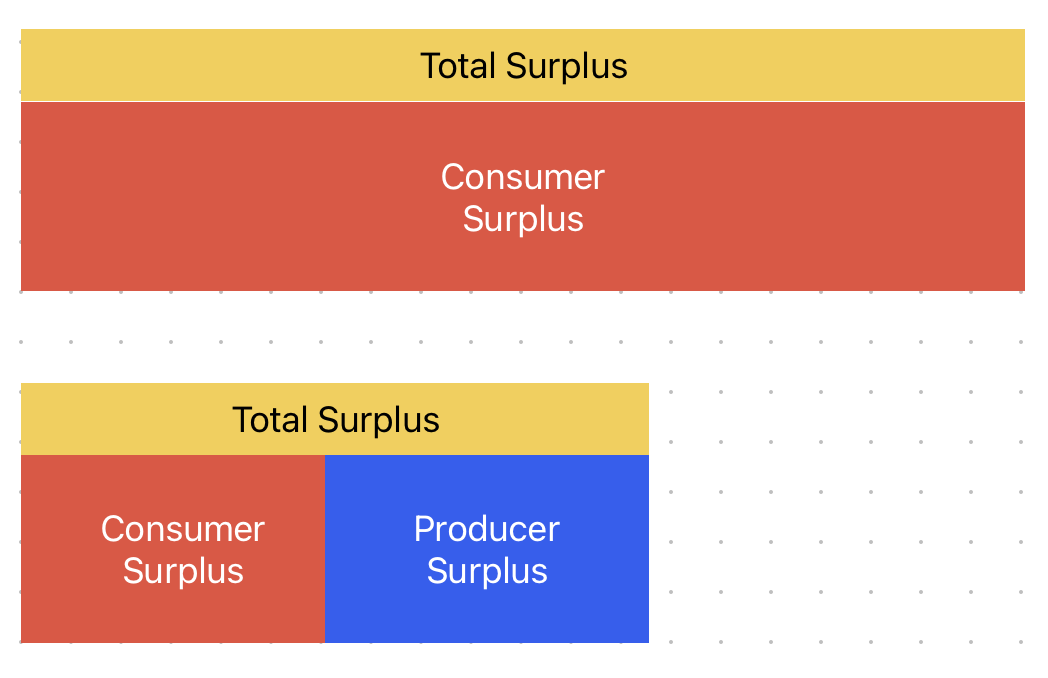
\includegraphics[width=0.70\linewidth]{graphics/TotalSurplus.png}
            \caption{Visual representation of TS, \textcolor{BrickRed}{\textbf{CS}} and \textcolor{MyBlue}{\textbf{PS}} in case of perfect competition (above) and monopolistic competition (below)}
            \label{fig:TotalSurplus}
        \end{figure}

        The difference is the deadweight loss. Some empirical studies claim that DWL is small, but they somehow misrepresent the negative effects associated with cartels/monopolies.\sn{\Remark{
        \textbf{Cartels} \(\Rightarrow\) negative effect in the long run over investments and innovation (cartelists are not allowed to be disruptive, make investments or increase capacity because these strategies would threaten cartels’ stability and eventually lead these cartels to break).
        }}

        

        \subsubsection{Price-Fixing Overcharges (2014)}

            in a huge - but also criticized – paper reviews 700 published economic studies and judicial decisions that contain 2,041 quantitative estimates of overcharges of hard-core cartels. The primary findings are: 
            \begin{enumerate}
                \item the median average long-run overcharge for all types of cartels over all time periods is 23.0\%; 
                \item the mean average is at least 49\%; 
                \item overcharges reached their zenith in 1891-1945 and have trended downward ever since; 
                \item median overcharges of international-membership cartels are 38\% higher than those of domestic cartels.
            \end{enumerate}

        \subsubsection{Efficient Monopoly}

            \begin{itemize}
                \item Prices are lower than in monopoly; 
                \item Quantities are grater than in monopoly.
                \item TS is clearly greater than in monopoly. Now we have a trapezoid $NewMC-D-EEM-L$ which is bigger than the trapezoid $MC-S-EM-PM$.
                \item Thus, in terms of $TS$, \textbf{Efficient Monopoly is better than Monopoly}. If we call TS in an efficient monopoly equilibrium “$TSEM$”, we have that: $TSEM > TSM$;
                \item Furthermore, if the area of the trapezoid in the efficient monopoly equilibrium is bigger than the area of the triangle representing \textcolor{BrickRed}{\textbf{CS}} in PC, than the size of the cake is increased, i.e., $TSEM$ is bigger of $TSCM$. Thus, apart from redistributive effects the net allocative effect could be positive.\sn{\Remark{
                \begin{itemize}
                    \item $TSEM > TSM$
                    \item $TSEM$ can be > or < than $TSCP$, depending, among other things, on the size of efficiency gains.
                \end{itemize}
                }}
            \end{itemize}

            \begin{figure}[h]
                \centering
                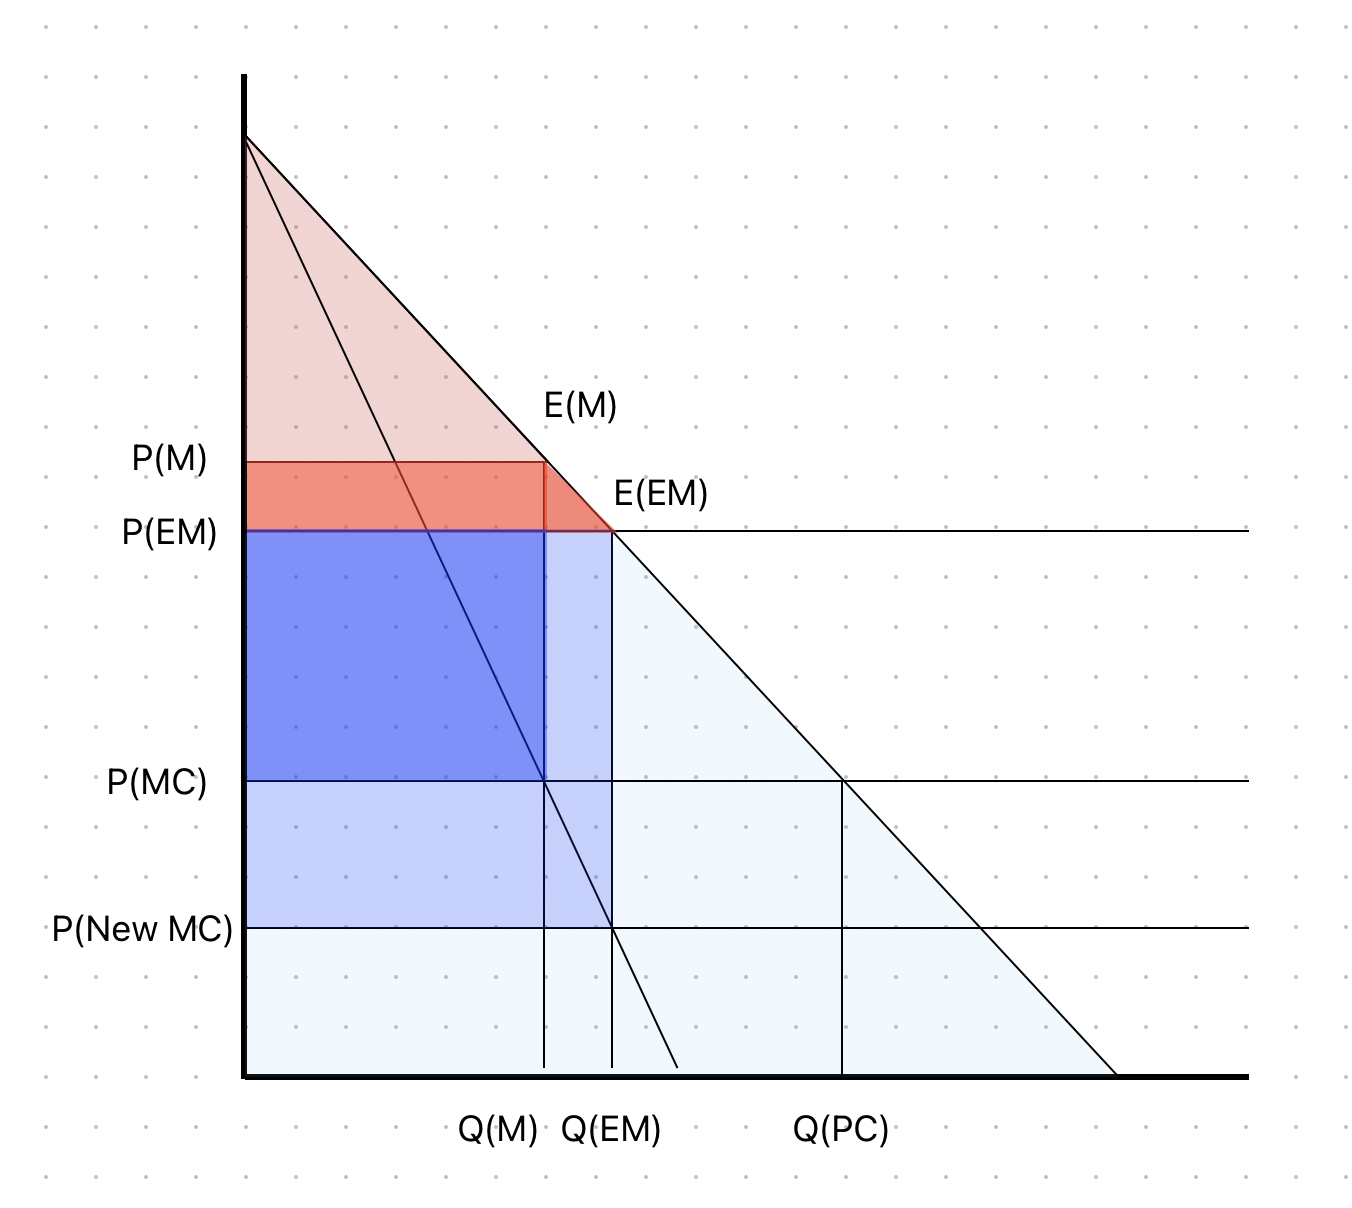
\includegraphics[width=0.66\linewidth]{graphics/EfficientMonopoly.png}
                \caption{Visual Representation of the different surpluses arising from the establishment of an efficient monopoly}
                \label{fig:efficient_monopoly}
            \end{figure}

    \subsection{A General Point}
    
        When anticompetitive effects due to mergers and agreements also produce efficiencies, there are no shortcuts (safe harbours, automatic prohibitions, per se rules), but AA must carefully study the combined, positive and negative, effects of the practices into consideration (usually with a counterfactual). 
        
        Suppose you must appraise a merger proposal. Thus, you must compare 2 alternative, future scenarios: A (in which the merger occurred) and B (in which no merger occurred).
        \begin{enumerate}
            \item[i.] If A is better than B, you should allow the parties to merge;
            \item[ii.] if B is better than A, the merger could be considered unlawful and should be blocked (it also depends on the relevance of the worsening of the economic situation post merger).
        \end{enumerate}
        In Europe, as we will discuss later, \textcolor{BrickRed}{\textbf{CS}} is the lead indicator of the competitive impact of a merger.
    
        \Note{
        Let’s close the parenthesis and go back to the initial question: \textbf{How do competition authorities know whether the market is functioning well?}
        }

\section{The natural development path of a market, firm practices and enforcement}

    AA endorse the main thesis of the perfect competition model: the higher the market power a firm (or a group of firms) holds, the higher the costs the market produces in terms of static efficiency (see the Dead Weight Loss) and in terms of income distribution (see the Distributive Effect in detriment of Consumers).

    \begin{figure}[h]
        \centering
        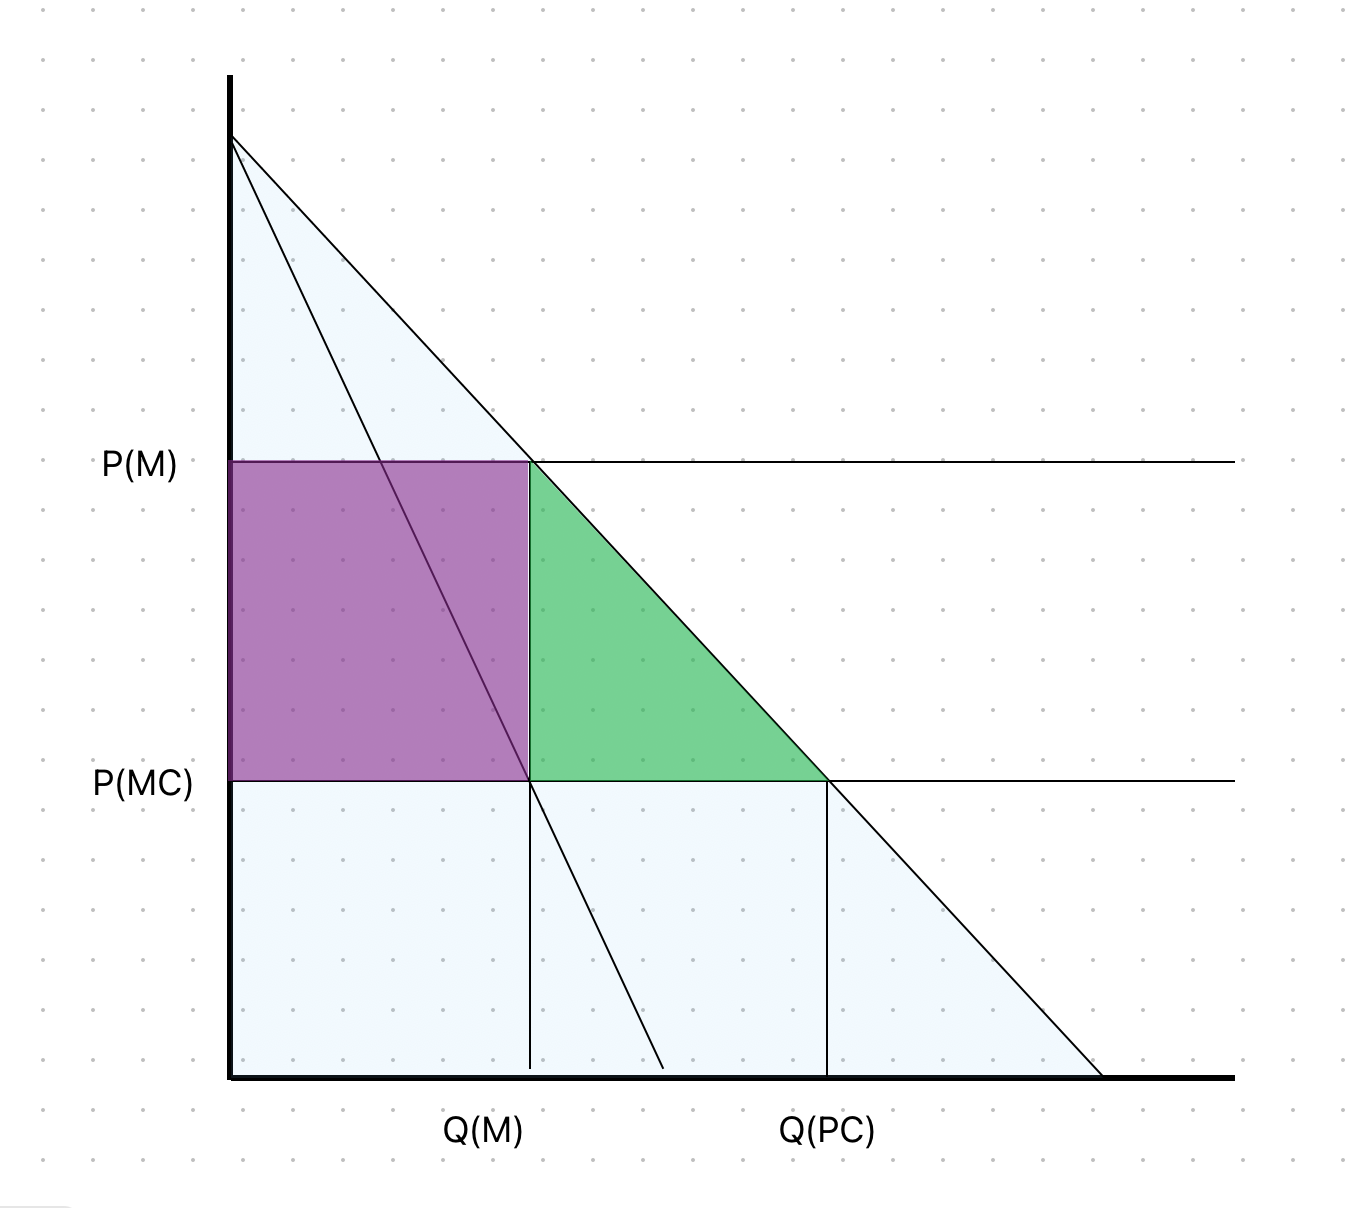
\includegraphics[width=0.68\linewidth]{graphics/DistributiveEffect_DWL.png}
        \caption{Visual representation of the Distributive Effect (purple) and the DeadWeight Loss (green)}
        \label{fig:DistribEffect_DWL}
    \end{figure}

    \begin{itemize}
        \item Competition authorities believe that firms are worsening market well-functioning when their practices limit output and increase market price! (These are called the“short run effects”). 
        \item Thus, competition law forbids those practices that may REDUCE market output and increase market price, just because these practices (are assumed to) drive the market away from a better state of the world (absent efficiencies).
        \item Let’s test this statement!
    \end{itemize}

    \begin{figure}[h]
        \centering
        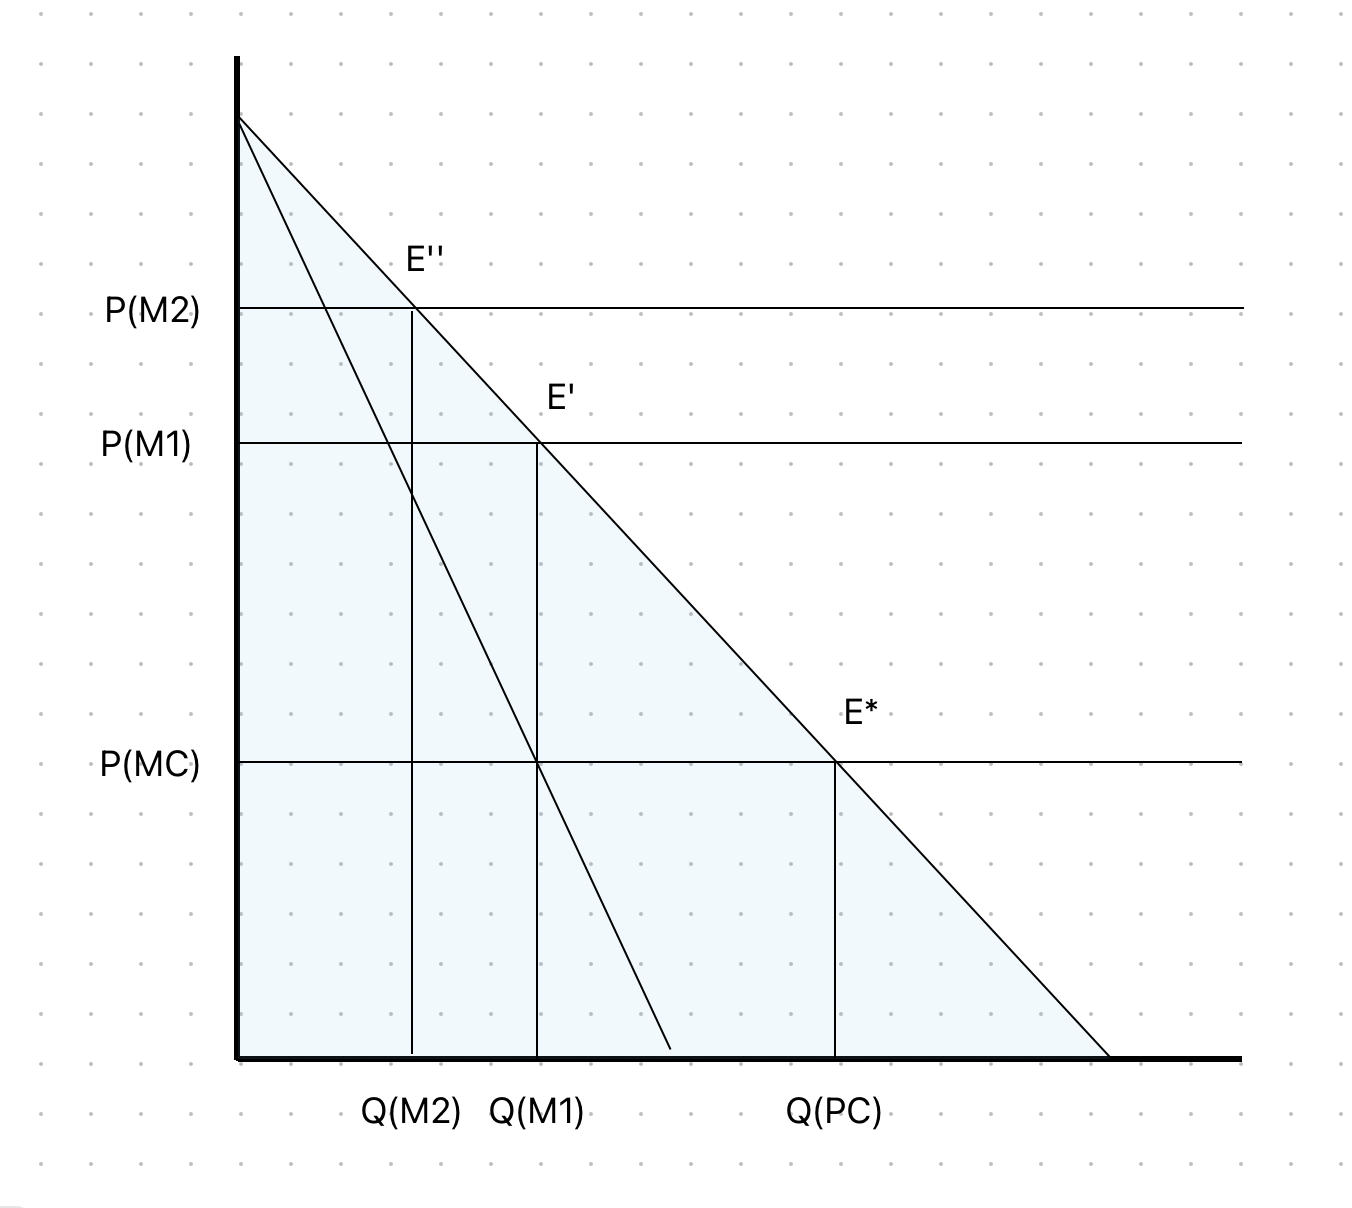
\includegraphics[width=0.80\linewidth]{graphics/DifferentMonopolies2.png}
        \label{fig:different_monopolies}
    \end{figure}

    \begin{itemize}
        \item[Case 1.] Suppose that in t0 the market is in \(E'\), which is not \(E^*\), i.e., the equilibrium of perfect competition
            \begin{itemize}
                \item Should antitrust law act to drive the market to \(E^*\)?
                    \(\Rightarrow\) \textbf{No}
            \end{itemize}
        \item[Case 2.] In $t1$ some firms’ practices bring the market to \(E''\)
            \begin{itemize}
                \item Should antitrust law forbid them? \(\Rightarrow\) \textbf{Yes}
            \end{itemize}
    \end{itemize}

    \begin{itemize}
        \item If the initial state of the market is $E’$, antitrust law is not supposed to drive the market back, towards $E^*$. Antitrust law protects actual/real competition. It does not work to recreate perfect competition, i.e., to reproduce the outcome of the perfect competition model by remedying to the many imperfections (such as externalities, barriers to entry, information asymmetries) that characterize real markets. This last job is left to economic regulators and legislators (even if sometimes… antitrust enforcers try to push and/or substitute the legislator).
        \item What triggers antitrust enforcement are practices that drive the market towards an equilibrium that is worse than the initial one. In our example, $E’’$ is worse than $E’$, because in $E’’$ the output is lower ($y’’<y’$) and prices are higher ($p’’>p’$). Thus, competition law must forbid those practices because, by altering the functioning of the market, they limit output and raise prices. \sn{\Remark{Competition law does not protect low prices and high amounts of output \textit{per se} (i.e., as such). Competition law uses the levels of prices and output to “understand” how the market is working/changing because of a merger/agreement.}}
    \end{itemize}

    NCAs don’t intervene to (try to) change the sketched development, if the change is due to “natural” reasons (market entry/exit, bankruptcy, investment in unrelated markets, etc.).

    \begin{itemize}
        \item The evolution from $T2$ to $T3$ may worsen \textcolor{BrickRed}{\textbf{CS}} but until it is notdue to a firm’s restrictive practice, no enforcement is triggered;
        \item NCAs enforce the law IFF firms’ restrictive practices induce a non transitory, significant “deviation” from the natural path that worsen \textcolor{BrickRed}{\textbf{CS}}.
    \end{itemize}

    \begin{figure}[h]
        \centering
        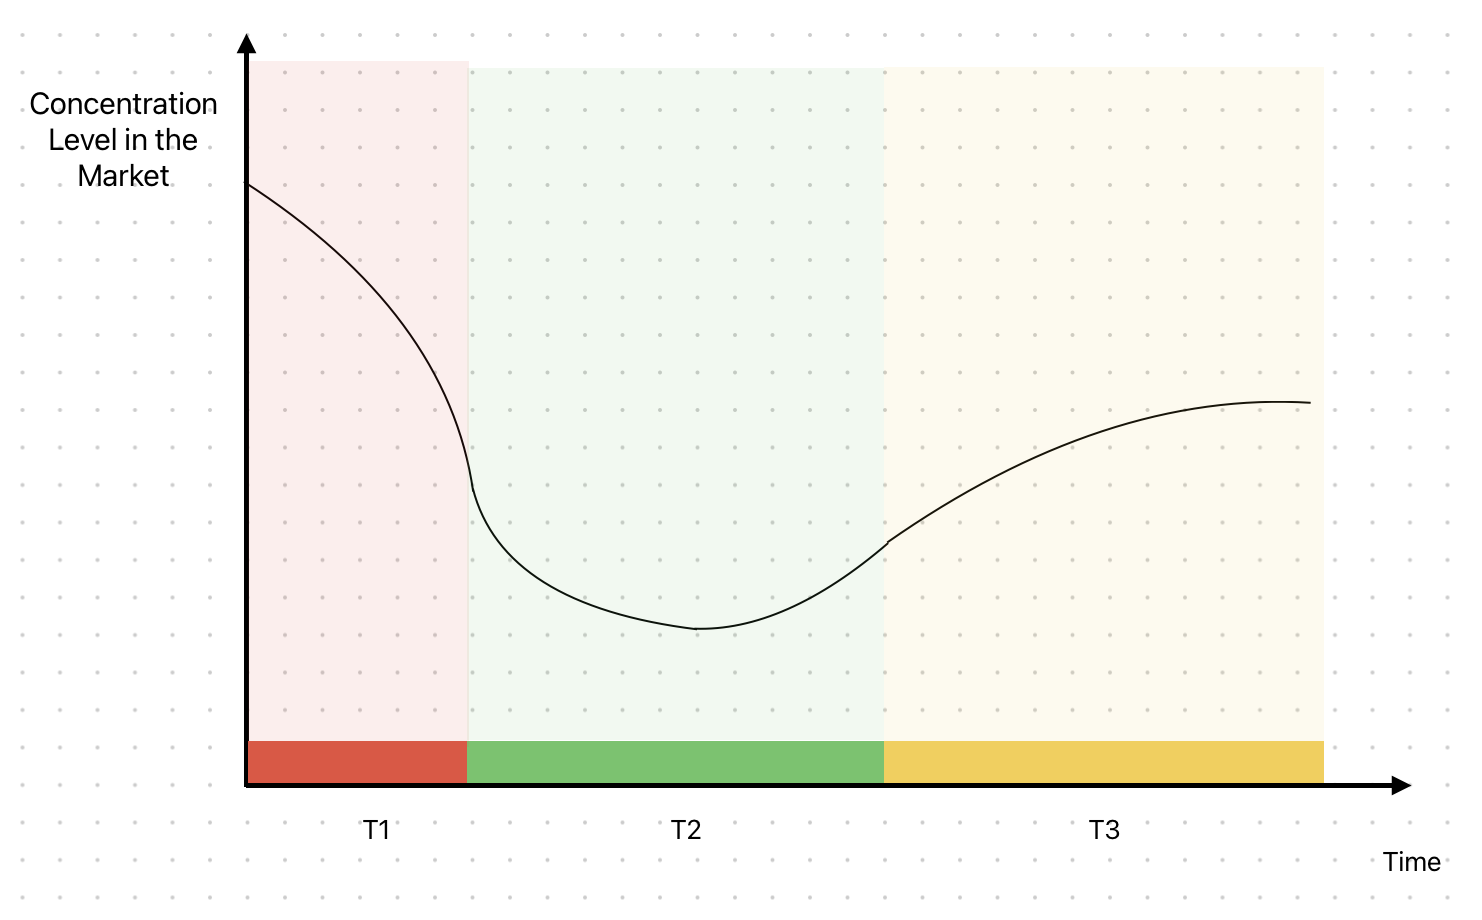
\includegraphics[width=0.85\linewidth]{graphics/Market_evolution.png}
        \caption{Natural Development Path of Market X}
        \label{fig:nat_dev_path_mkt}
    \end{figure}

    \begin{figure}[h]
        \centering
        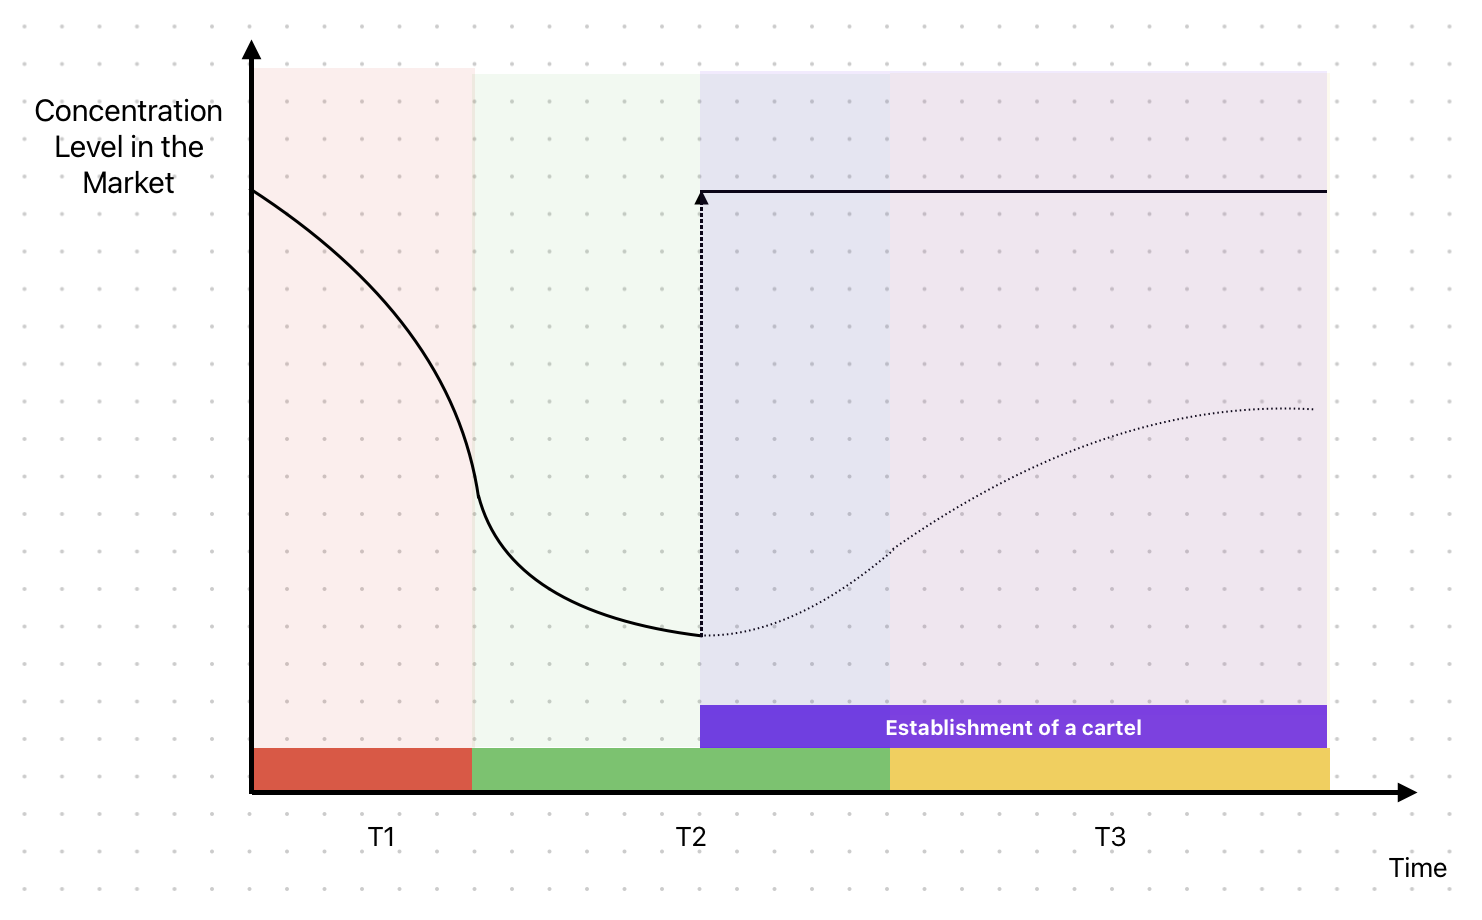
\includegraphics[width=0.85\linewidth]{graphics/establishment_cartel.png}
        \caption{Development of Market Concentration in the presence of a monopolistic cartel}
    \end{figure}

    \Note{“Antitrust enforcement is not like a family doctor who prescribe on a daily basis some drugs to prevent ageing; in contrast, antitrust is like a medical surgeon who intervenes with the scalpel to eradicate the illness only when it finds a very acute disease”}

    \begin{itemize}
        \item Furthermore, antitrust institutions endorse economic theories showing that, over the long run:
            \begin{itemize}
                \item consumers benefit from varied and good products, that is, from increasingly larger ranges of products of better quality and
                \item innovation increases CS much more than any policy aimed at pushing prices down to marginal costs.
            \end{itemize}
        \item Therefore, antitrust law also forbids practices unduly reducing product quality, consumers’ choice (that is, product variety), and innovation (“long run effects”)
        \item In practice, many cases are decided based on short run effects. Yet sometimes (for example, when inventions/patent/R\&D are involved) long run effects are taken into consideration.
        \item In cases of conflicts, often (not always) the effects on innovation are deemed more important than effects on market output and price. For example, the practices promoting innovation are deemed lawful even when they make market price increase. 
    \end{itemize}

    \subsection{In summary}

        A behaviour that may worsen market well-functioning is a behaviour that may harm consumer welfare over the short and long run, that is, a practice that may:

        \begin{itemize}
            \item In the short run:
                \begin{itemize}
                    \item increase market price
                    \item reduce market output
                    \item worsen product quality
                \end{itemize}
            \item In the long run:
                \begin{itemize}
                    \item worsen product variety
                    \item lower innovation rate
                \end{itemize}
        \end{itemize}

        \Note{Competition law aims at preventing these practices!}

    \subsection{The End on Ambiguous Practices}

        \begin{itemize}
            \item HP: a merger leads from perfect competition to efficient monopoly. In that circumstance:
                \begin{itemize}
                    \item $TSEM > TSM$, while it is difficult to state whether $TSEM$ is larger or smaller than $TSPC$.
                \end{itemize}
            \item If $TSEM > TSPC$, but $CS_{effm} < CS_c$, can we allow the agreement/merger ?
            \item i.e., how can we judge a situation in which the size of the cake becomes bigger, but at the same time the slice that goes to consumers is thinner ?
            \item In the past we observed a divergent approach in the EU from the US attitude toward efficiency enhancing behaviour.
        \end{itemize}

        \subsubsection{In the European doctrine}

            In EU, we look at CS variations; Article 101(3) exemption can be applied \textbf{IFF}: the agreement
                \begin{itemize}
                    \item “does not afford such undertaking the possibility of eliminating competition in respect of a substantial part” of the market, and
                    \item the “agreement allows consumers a fair share of the resulting benefit”.
                \end{itemize}

        \subsubsection{In the Chicagoan doctrine}

            The goal is TW (the size of the cake). Why? For many legitimate (at least in theory) reasons:
                \begin{itemize}
                    \item[a.] You can always rebalance the redistributive effects with fiscal policy, and wealth transfers;
                    \item[b.] in the US, consumers are usually also shareholders. Thus, they earn with one hand (in form of dividends) what they may have lost with the other one (in terms of decreased consumer welfare). And by definition the net effect is positive.
                \end{itemize}
